\section{Language}\label{sec:language}
This section describes the domain specific language built upon the language model described in Section~\ref{sec:model}. First the deployment of the language is provided that explains how the DSL is operates and is used in usage management systems. This is followed by a detailed example of the syntax and semantics, and major components of the language. Finally, we demonstrate how the language can be extended to include different types of evaluators deploying different types of logics. 

\begin{figure}[!t]
\centering
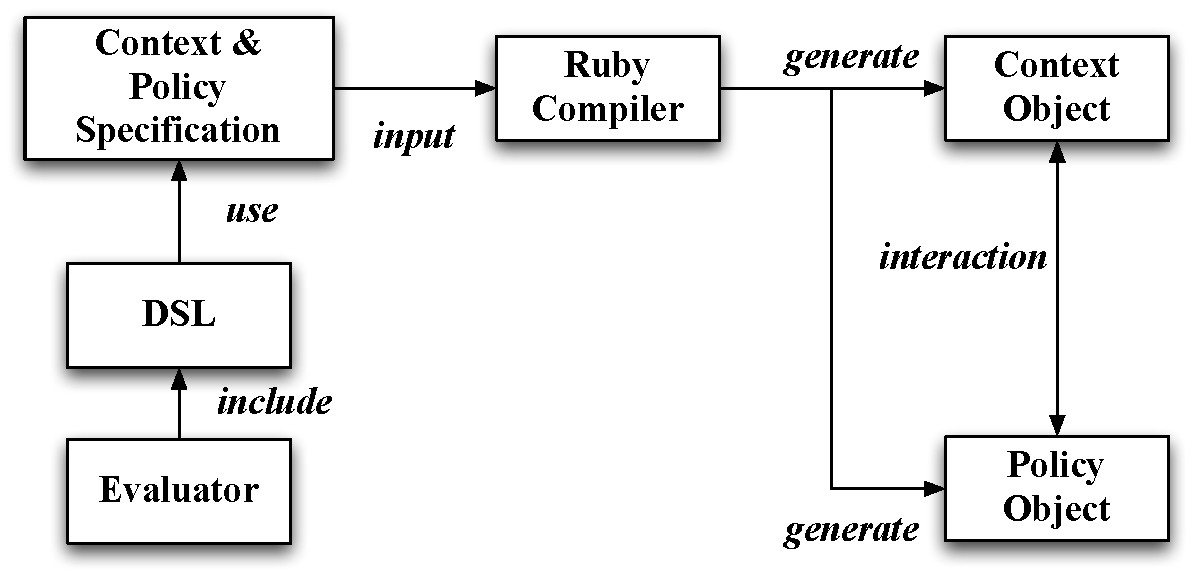
\includegraphics[width=3.5in]{DSL-usage}
\caption{The role of DSL in usage management systems}
\label{fig:DSL-usage}
\end{figure}

\subsection{Language Operation}
The use and operation of the DSL for usage management is shown in Figure~\ref{fig:DSL-usage}. The DSL provides a language for specification of contexts and policies as described in the previous section. As shown in the figure, the DSL can incorporate different types of evaluators for expression of different types of usage semantics. A DSL, along with an appropriate evaluator is then used to specify contexts and policies. Users are allowed to choose from different types of evaluators that provide the right type of semantics needed by the users. The policy specification and context specification, described using the DSL is then taken by a Ruby compiler to generate a corresponding context and policy object. In usage management systems, context objects are generated on the client side and maintained within the computing platform. The policy specification is provided by the resource owners, is converted into a policy object. Following this, the policy and context objects interact with each other and operate within a usage management system.  

\subsection{Language Description}
The language is based on the model description provided in the previous section, and enables specification of the various policy semantics and context descriptions. 

\subsubsection{Context Specification}

The DSL provides a mechanism for specification of different types of contexts based on the context structure explained in the previous section. A context consists of a set of entities, such as Subject, Resource, and Environment, and each of these entities possess a set of properties. Every property supports a set of functions that operate over the property. The steps involved in defining a context first includes the description of different types of properties. The properties are then allocated to different entities, and then entities are assigned to a given context. 

\begin{table*}[t]
\caption{An example structure of context.}
\label{table:context}
\begin{center}
%{\small
\begin{tabular}{|c|c|c|c|}
\hline
\multicolumn{4}{|c|}{ \bf Context}\\
\hline
{ \bf Entity} & {\bf Property ($p$)} & { \bf Domain ($D_p$)} & {\bf Functions ($F_p$)}\\
\hline
\multirow{3}{*}{Environment (E)} & OperatingSystem & \{Windows, OSX, SELinux\}&  equatable\\
                                                    & Device & \{Workstation, Handheld, Blackberry, Terminal\} & equatable \\
                                                    & SecurityDomain & \{ ABNet, SECNet, TELNet, OMNINet\} & comparable\\ 
\hline
\multirow{3}{*}{Subject (S)} & SecurityClearance & \{Top Secret, Secret, Confidential\} &  comparable\\
				      &Project & \{Zebra, Yuma, Lion\} & equatable\\
				       &Role & \{Alpha, Beta, Delta\} & equatable\\

\hline
 Resource(R) & SecurityClassification & \{ Top Secret, Secret, Confidential, Unclassified\} & comparable \\
\hline

\end{tabular}
%}
\end{center}
\label{default}
\end{table*} 

Consider a multi-level security context as shown in Table~\ref{table:context}. The context consists of two entities, namely, {\em Subject} and {\em Environment} and {\em Resource}. {\em Subject} entity has three properties, namely, {\em Security Clearance}, {\em Role} and {\em Project}. {\em Environment} entity has three properties, namely, {\em OperatingSystem}, {\em Device} and {\em SecurityDomain}. {\em Resource} entity has one property, {\em SecurityClassification}. Every property supports a set of functions depending on the type of that property. For the purpose of this discussion, we explain two types of properties, namely, equatable and comparable. Equatable properties primarily support equality functions  ``$=$" and ``$!=$". Comparable properties support functions that allow relative comparison of two values, namely, ``$=$" , ``$!=$", ``$<$", ``$>$",  ``$\leq$", ``$\geq$" and ``$between()$". Both, equatable and comparable property types support ``$get()$" and ``$set()$" functions to retrieve and set property values. The properties {\em OperatingSystem}, {\em Device}, {\em Project} and {\em Role} are equatable properties, and {\em SecurityDomain}, {\em SecurityClearance} and {\em SecurityClassfication} are comparable properties. {\em SecurityDomain} property values have the ordering $ABNet > SECNet > TELNet > OMNINet$,  {\em SecurityClearance} property values have the ordering $Top\;Secret > Secret > Confidential$, and {\em SecurityClassification} property values have the ordering $Top\;Secret > Secret > Confidential > Unclassified$. 

In order to specify this context, individual properties are defined first as follows. 

\begin{tabbing}
             Property \= (:OperatingSystem) {\bf do} \\
\>	   {\bf values}  :Windows, :OSX,  :SELinux\\
\>	   {\bf functions}   :set, :get, :equatable \\
	{\bf end} 
\end{tabbing}
	
\begin{tabbing}
 Property \= (:Device) {\bf do} \\
\>	 {\bf values} \= :Workstation, :Handheld, :Blackberry, \\
\>\>      :Terminal\\
\>	 {\bf functions}  :set, :get, :equatable \\
	 {\bf end}
\end{tabbing}

\begin{tabbing}
Property \= (:Project) {\bf do} \\
\>	 {\bf values}  :Zebra, :Yuma, :Lion\\
\>	 {\bf functions} :set, :get, :equatable \\
	 {\bf end}
\end{tabbing}

\begin{tabbing}	
 Property  \= (:Role) {\bf do} \\
\>	 {\bf values} :Alpha, :Beta, :Delta\\
\>	 {\bf functions}  :set, :get, :equatable \\
	 {\bf end}
\end{tabbing}
	
In this example, classes  {\em OperatingSystem, Device, Project} and {\em Role} that inherit the type {\em Property} are specified. The term {\em values} specify the set of valid values and {\em functions} define the set of functions supported by the class as described earlier. Similarly, classes for comparable properties are defined, with the addition that the ordering of the valid values is specified by the user as shown below. 

\begin{tabbing}
             Property \= (:SecurityDomain) {\bf do} \\
\>	   {\bf values}  :ABNet, :SECNet, :TELNet, :OMNINet\\
\>	   {\bf functions}   :set, :get, :comparable \\
\>	   {\bf order} :ABNet > :SecNet > :TELNet > :OMNINet\\
	{\bf end} 
\end{tabbing}
	
\begin{tabbing}
 Property \= (:SecurityClearance) {\bf do} \\
\>	 {\bf values} \= :Top Secret, :Secret, :Confidential \\
\>	 {\bf functions}  :set, :get, :comparable \\
\>       {\bf order} :Top Secret > Secret > Confidential
	 {\bf end}
\end{tabbing}

\begin{tabbing}
Property \= (:SecurityClassification) {\bf do} \\
\>	 {\bf values} \=  :Top Secret, :Secret, :Confidential, \\
\>\>                               :Unclassified\\
\>	 {\bf functions} :set, :get, :comparable \\
\>       {\bf order} \= :Top Secret > :Secret > :Confidential > \\
\>\>                           :Unclassified\\
	 {\bf end}
\end{tabbing}

In this example, classes {\em SecurityDomain}, {\em SecurityClearance} and {\em SecurityClassification} that inherit the type {\em Property} are generated. Each of these classes are comparable and provide a set of comparison functions. The {\em order} keyword allows context designers to specify the value ordering in an easy manner. The property classes defined here are now assigned to the entities {\em Subject}, {\em Resource} and {\em Environment}. These assignments are described in the DSL as follows. 

\begin{tabbing}
 Entity \= (:Subject) {\bf do} \\
\>	 {\bf contains} \=  :Project, :Role, :SecurityClearance \\
	 {\bf end}
\end{tabbing}

\begin{tabbing}
 Entity \= (:Environment) {\bf do} \\
\>	 {\bf contains} \=  :Device, :OperatingSystem,\\
\> \>                                 :SecurityDomain \\
	 {\bf end}
\end{tabbing}

\begin{tabbing}
 Entity \= (:Resource) {\bf do} \\
\>	 {\bf contains} \=  :SecurityClassification \\
	 {\bf end}
\end{tabbing}

The above specification generates the {\em Subject}, {\em Resource} and {\em Environment} classes. The DSL generates a {\em Subject} class that contains properties of type {\em Role}, {\em Project}, and {\em SecurityClearance}. Entity type classes, by default, provide functions that provide information about the  properties contained in these entities. Finally, each of these entities are included in the context, which in this case is a multi-level security context. The syntax for context specification is as follows. 

\begin{tabbing}
 Context \= (:MultilevelSecurity) {\bf do} \\
\>	 {\bf contains} \=  :Subject, :Resource, :Environment \\
	 {\bf end}
\end{tabbing}

This specification generates the {\em MultilevelSecurity} class that contains entities {\em Subject}, {\em Resource} and {\em Environment}. The process of context specification is carried out by context designers. This a less frequently carried out process, and the DSL provides an easier way to provide this specification. The {\em MultilevelSecurity} class is instantiated, and the corresponding object of this class is maintained on the client system. The property values maintained by this object defines the circumstances under which activities are carried out in the client system. 

It must be noted that various kinds of properties can be described using this method. For example, properties having set-based characteristics can be defined that support set functions such as ``$in()$" to determine if a given element is a part of the set. 

The context generated in this manner is then used to define policies. The DSL provides a policy specification component that provides an easy way to specify policies. Policy specification are read by the Ruby interpreter and converted into policy objects. For example, consider the following policy. 

{\em ``A document with a security classification greater than or equal to Secret can only be viewed by subjects working on project Yuma having security clearance greater than or equal to Secret on only Blackberry devices operating in security domain greater than SECNet . Also, viewing can be done only after project Yuma has been project-authorized. "}

The above policy is expressed in terms of the DSL in the following steps. 

\begin{tabbing}
a1= \= activity (view) {\bf do} \\
\>	constraint\_evaluators :propositional\\
\>	SecurityClassification $\geq$ Secret $\wedge$ Project $=$ Yuma $\wedge$\\
\>	SecurityClearance $\geq$ Secret $\wedge$  Device $=$ Blackberry $\wedge$ \\
\>	SecurityDomain $\geq$ SECNet \\
{\bf end}
\end{tabbing}

First an activity {\em view} is defined and associated with the constraints defined in terms of context properties described earlier. Such activities with restrictions are called {\em restricted activities} as described in the language model. It must be noted that the activities defined in the DSL are agreed upon {\em a priori} with the client system. Now we define another activity, {\em project-authorization} along with its restrictions (or constraints)

\begin{tabbing}
a2= \= activity (project-authorization) {\bf do} \\
\>	constraint\_evaluators :propositional\\
\>	 Project $=$ Yuma \\
{\bf end}
\end{tabbing}

Once activities activities $a1$ and $a2$ are defined, relationship between the two activities is defined. Such relationships are called usage policies, and are defined the policy definition of the DSL. Usage semantics establish relationships among different activities along with behavioral or or history-based characteristics such as count limits on a given activity. In the present form, the DSL allows permissions, obligations and count limits. However, the DSL can be extended, and usage semantics can be added or changed by using different types of evaluators. This aspect of the DSL is discussed later. In this example, activity {\em view} is a permission, and activity {\em project-authorization} is an obligation for exercising this permission. These semantics are expressed in the DSL as follows. 

\begin{tabbing}
pol = \= policy a1, a2 {\bf do} \\
\>	policy\_evaluators :standard \\
\>	permit \= a1 {\bf do} \\
\>\>		when a2 \\	
\>	{\bf end} \\
{\bf end} \\
\end{tabbing}

The above policy specification says that the policy {\em pol} is defined using activities {\em a1} and {\em a2}, and activity {\em a1} is a permission that is obligated by activity {\em a2}.  Additional usage semantics could be added to this activity, for instance count-based limits as follows. 

\begin{tabbing}
pol = \= policy a1, a2 {\bf do} \\
\>	policy\_evaluators :standard \\
\>	permit \= a1 {\bf do} \\
\>\>		when a2 \\	
\>	{\bf end} \\
\> 	count\_limit a1, 5 \\
{\bf end} \\
\end{tabbing}

Once the policy specification is provided to the Ruby interpreter, it converts it into a policy object. A policy object is nothing by an executable ruby object with a well-defined policy interface. An example interface provided by the standard policy evaluator defined here contains the following set of functions. 

\begin{itemize}
\item {\bf permissions?()} Returns the set of permissions for a given policy.
\item {\bf obligations?(a)} Returns the set of all obligations associated with a given permission. 
\item {\bf remaining\_obligations(a)} Returns the set of remaining obligations for a given permission. 
\item {\bf remaining\_count(a)} Returns the set of remaining count for a given permission. 
\item {\bf allowed?(a, ctx)} A boolean function that returns {\em true/false} whether a given activity can be carried out under a given context. 
\item {\bf reset()} Resets the policy by resetting its state. 
\end{itemize}

The policy DSL proposed here is simply a skeleton which can extended by incorporating different types of logics expressing various usage semantics. The manner in which these extensions may be carried out is described next. 

\subsection{Langauge Extensions}

The DSL allows inclusion of different types of evaluators that provide users with different sets of usage semantics. The evaluators provide a design space for innovation and extensibility. In the examples provided here, the evaluators used for evaluating constraint (or restriction) semantics is a {\em propositional} evaluator. This evaluator allows constraints to be expressed as boolean formulas constructed from property functions. This evaluator provides a design space for expressing restrictions in terms of context properties. This evaluator is merely a pulugin that can be replaced by a different constraint evaluator that allows constraints to be expressed in a different manner. 

Similarly, the policy construct uses a policy evaluator for expressing and reasoning about usage semantics. The {\em standard} evaluator used here allows expression of permissions, obligations and count-based limits. The usage semantics is similarly a design space where different types of evaluators can be used to express various types of usage semantics such as parallel actions, partial ordering, and interleaving semantics among others. 

In the next section we show how different rights expression languages such as ODRL, XrML and creative commons can be mapped on to this DSL. 




